%!TEX root = ../main.tex

\noindent
Στο κεφάλαιο \ref{ch:chap2} αναλύθηκε με λεπτομέρεια το θεωρητικό υπόβαθρο στο οποίο βασίστηκε η εργασία. Εδώ περιγράφεται η προσέγγιση που επιλέχθηκε για την επίλυση του προβλήματος της εκτίμησης DOA μέσω αμφιωτικών παραμέτρων. Αρχικά προσεγγίζεται η δημιουργία των σημάτων θορύβου που χρησιμοποιήθηκαν για την εκπαίδευση των μοντέλων, στη συνέχεια η διαδικασία κατασκευής των αμφιωτικών σημάτων μέσω BRIR, καθώς και η εξαγωγή των διωτικών παραμέτρων με το μοντέλο dietz2011. Έπειτα περιγράφεται η καινούρια μέθοδος συμπίεσης των αμφιωτικών παραμέτρων που υλοποιήθηκε για τους σκοπούς αυτής της εργασίας, καθώς και η επιπλέον προεπεξεργασία των δεδομένων προτού αυτά χρησιμοποιηθούν για την εκπαίδευση των διάφορων μοντέλων. Αναλύονται επίσης οι διάφορες αρχιτεκτονικές που χρησιμοποιήθηκαν, καθώς και οι μετρικές που είναι απαραίτητες για την αξιολόγηση των μοντέλων. Τα μοντέλα δοκιμάστηκαν για δειγματοληψία $44.1\; kHz$.

\section{Σήματα εισόδου} \label{sec:input_signals}

\noindent
Τα πηγαία σήματα που χρησιμοποιήθηκαν για την εκπαίδευση των NN ήταν 'εκρήξεις' (bursts) λευκού θορύβου, ο οποίος έχει χαρακτηριστικά που περιγράφονται στην υποενότητα \ref{sec:white_noise}. Συνολικά η διάρκεια κάθε σήματος ήταν $200 ms$. Στην περίπτωση της δειγματοληψίας με $f_s = 44.1 kHz$ αυτό αντιστοιχεί σε 8820 δείγματα. Οι εκρήξεις είχαν μεταβλητή διάρκεια $3 - 170 ms$ με τυχαίο τρόπο. Τυχαίο ήταν επίσης το σημείο εκκίνησης της κάθε έκρηξης στο συνολικό σήμα. Δημιουργήθηκαν συνολικά 29 τέτοια σήματα και η γενική περιγραφή κάθε σήματος φαίνεται στην εξίσωση \ref{eq:input_signals}, όπου $Z_n \sim N(0,P)$ δηλαδή μια κανονική κατανομή με μέση τιμή μηδέν και διακύμανση-ισχύ \textit{P}.

\begin{CEquation}
\begin{split}
         Sig_in(n) = 
         \begin{cases}
         Z_n, & n_{start} < n < n_{end}\\
         0, & \text{αλλού}
         \end{cases}   
         \label{eq:input_signals}
\end{split}
\end{CEquation}

Μερικά από τα σήματα εισόδου φαίνονται στο Σχήμα \ref{fig:input_signals_examples}. Μετά την δημιουργία τους κανονικοποιούνται στο κλειστό διάστημα $amplitude = [-1, 1]$, ώστε τελικά να αποθηκευτούν σε μορφή wav για μελλοντική χρήση. Η διάρκεια των σημάτων καθορίστηκε στα $200 ms$, προκειμένου να διατηρηθεί σχετικά μικρό το διάνυσμα εισόδου στο NN, αλλά και να προλάβει να επέλθει η σταθερή κατάσταση μετά τη μεταβατική κατάσταση (transient) που δημιουργείται στην έναρξη και την παύση του σήματος, αφού κρίθηκε πως αυτό έχει ιδιαίτερη σημασία στον τρόπο που αντιλαμβάνεται ο άνθρωπος τον ήχο, και άρα να τροφοδοτηθεί το NN, με δεδομένα που έχουν υψηλή συγκέντρωση χρήσιμης πληροφορίας.

\begin{figure}[h]
  \centering
  \includegraphics[width=\textwidth]{images/bursts.png}
  \caption{Σήματα λευκού θορύβου που χρησιμοποιήθηκαν ως είσοδος στο μοντέλο.}
  \label{fig:input_signals_examples}
\end{figure}



\section{Δημιουργία αμφιωτικών σημάτων} \label{sec:bin_sig_creation}

\noindent
Τα σήματα που περιγράφονται στην υποενότητα \ref{sec:input_signals} στη συνέχεια συνελίσονται με BRIRs, για διαφορετικές γωνίες, που προέρχονται από τρία δωμάτια: Το TU Berlin Auditorium 3 \cite{Wierstorf2016b}, το Spirit \cite{Wierstorf2016a}, και το Calypso \cite{Wierstorf2016}. Σε κάθε περίπτωση, το ανδρείκελο απείχε 1m από την πηγή, ενώ έγιναν μετρήσεις με ανάλυση $1^o$ στο οριζόντιο επίπεδο, από $-90^o$ μέχρι $+90^o$ χρησιμοποιώντας το ανδρείκελο KEMAR και ηχεία Genelec, τοποθετημένα σε ανύψωση $0^o$. 

Στην εργασία αυτή χρησιμοποιήθηκε ανάλυση στο οριζόντιο επίπεδο $2^o$, με αποτέλεσμα να προκύψουν 91 κρουστικές για κάθε δωμάτιο. Χρησιμοποιήθηκαν και τα τρία δωμάτια, και άρα μετά από τη συνέλιξη κάθε ενός από τα 29 σήματα εισόδου, με μία από τις $3 * 91 = 273$ διαφορετικές κρουστικές, δημιουργούνται συνολικά $29 * 273 = 7917$ διαφορετικά σήματα εισόδου.

Αναλυτικότερα, αφού φορτωθεί το εκάστοτε dataset, και από αυτό διαβαστεί η BRIR, η οποία εμφανώς αποτελείται από δύο κανάλια διότι είναι binaural, εφαρμόζεται σε αυτή ένα παράθυρο Half Hanning μήκους 9000 δειγμάτων, αφού ρυθμιστεί η ζητούμενη δειγματοληψία. Τα δύο κανάλια της BRIR συνελίσονται με το mono σήμα εισόδου και προκύπτει το αμφιωτικό σήμα από το οποίο θα εξαχθούν στη συνέχεια οι αμφιωτικές παράμετροι. Έτσι, το αποτέλεσμα της συνέλιξης είναι ένα αμφιωτικό σήμα διαστάσεων $[2,L]$, όπου $L = M + N - 1 = 17819$, με δεδομένο ότι η BRIR έχει μήκος $M = 9000$ δείγματα και το mono σήμα μήκος $N = 8820$ δείγματα.

Η παραθύρωση έγινε λόγω περιορισμών στους υπολογιστικούς πόρους, αλλά επιλέχθηκε τέτοιο μέγεθος παραθύρου ώστε να διατηρούνται τα σημαντικότερα χαρακτηριστικά των BRIR. 

Μια κρουστική μαζί με το παράθυρο που εφαρμόζεται σε αυτή και η BRIR μετά την εφαρμογή του, φαίνονται στο Σχήμα \ref{fig:brir_processing}. Συνοπτικά η διαδικασία της δημιουργίας των αμφιωτικών σημάτων φαίνεται στο Σχήμα \ref{fig:binaural_signal_gen_block}.

\begin{figure}[h]
  \centering
  \includegraphics[width=\textwidth]{images/binaural_signal_gen_block.png}
  \caption{Δημιουργία αμφιωτικών σημάτων. Το block sub-sampling χρησιμοποιείται μόνο στην περίπτωση που τα σήματα έχουν διαφορετική δειγματοληψία από την επιθυμητή $f_s = 44.1 kHz$}
  \label{fig:binaural_signal_gen_block}
\end{figure}

\begin{figure}
     \centering
     \begin{subfigure}[b]{\textwidth}
         \centering
         \includegraphics[width=\textwidth]{images/brir_window.png}
         \caption{}
         \label{fig:brir_window}
     \end{subfigure}
     \hfill
     \begin{subfigure}[b]{\textwidth}
         \centering
         \includegraphics[width=\textwidth]{images/windowed_brir.png}
         \caption{}
         \label{fig:windowed_brir}
     \end{subfigure}
        \caption{(α'): BRIR και το αντίστοιχο Half Hanning παράθυρο, (β'): BRIR μετά την παραθύρωση. Τα σχήματα είναι για $f_s = 44.1 kHz$ }
        \label{fig:brir_processing}
\end{figure}

\section{Εξαγωγή αμφιωτικών παραμέτρων}

\noindent
Σε αυτή την ενότητα, αναλύεται η εφαρμογή του μοντέλου του Dietz το θεωρητικό υπόβαθρο του οποίου περιγράφεται στην υποενότητα \ref{sec:dietz_theory}. Η συνάρτηση είναι υλοποιημένη σε MATLAB, στο Auditory Modeling Toolbox. Η συνάρτηση χρειάζεται ως ορίσματα το binaural σήμα και τη συχνότητα δειγματοληψίας, ενώ στην έξοδό της δίνονται οι αμφιωτικές παράμετροι.

Συνοπτικά η διαδικασία που ακολουθείται για τον υπολογισμό των παραμέτρων, φαίνεται στο Σχήμα \ref{fig:dietz_block_diagram_MATLAB} και τα επιμέρους στοιχεία της αναλύονται στη συνέχεια.

\begin{figure}[h]
  \centering
  \includegraphics[width=\textwidth]{images/dietz_block_diagram_MATLAB.png}
  \caption{Συνοπτική περιγραφή της υλοποίησης του μοντέλου Dietz για το ακουστικό σύστημα.}
  \label{fig:dietz_block_diagram_MATLAB}
\end{figure}

\noindent
Αξίζει εδώ να σημειωθεί πως η υλοποίηση του μοντέλου, πιστώνεται στους:
\begin{itemize}
    \item Tobias Peters (tobias@medi.physik.uni-oldenburg.de)
    \item Mathias Dietz (mathias.dietz@uni-oldenburg.de)
    \item Martin Klein-Hennig (martin.klein.hennig@uni-oldenburg.de)
\end{itemize}{}

Παρακάτω, μελετάται η λειτουργία του μοντέλου, με βάση ένα  από τα binaural σήματα εισόδου που χρησιμοποιούνται, που αντιστοιχεί σε γωνία άφιξης $+80^o$ από το δωμάτιο Spirit, όπως φαίνεται στο Σχήμα \ref{fig:example_bin_sig}.

\begin{figure}[h]
  \centering
  \includegraphics[width=\textwidth]{images/example_bin_sig.png}
  \caption{Binaural σήμα για γωνία άφιξης $+80^o$, στο δωμάτιο Spirit.}
  \label{fig:dietz_out}
\end{figure}

\subsection{Φιλτράρισμα Μέσου Αυτιού}

Αρχικά, το σήμα περνά από ένα bandpass butterworth φίλτρο με $f_{c1} = 500 Hz$ και $f_{c2} = 2 kHz$ το οποίο φαίνεται στο Σχήμα \ref{fig:butterworth_dietz_1}, ενώ το τελικό αποτέλεσμα της επεξεργασίας φαίνεται στο Σχήμα \ref{fig:dietz_out1}. Όπως είναι αναμενόμενο, όντας ουσιαστικά σήμα λευκού θορύβου, η μορφή του αλλάζει αισθητά στο πεδίο του χρόνου, αφού μειώνεται σημαντικά το υψίσυχνο περιεχόμενο.

\begin{figure}[h!]
  \centering
  \includegraphics[width=\textwidth,height=8cm]{images/butterworth_dietz_1.png}
  \caption{IIR φίλτρο τύπου butterworth που προσομοιώνει το φιλτράρισμα του μέσου αυτιού.}
  \label{fig:butterworth_dietz_1}
\end{figure}

\begin{figure}[h!]
  \centering
  \includegraphics[width=\textwidth]{images/dietz_out1.png}
  \caption{Αποτέλεσμα της επεξεργασίας του μέσου αυτιού.}
  \label{fig:dietz_out1}
\end{figure}

\subsection{Προσομοίωση Εσωτερικού Αυτιού}

Σε αυτό το σημείο, για την προσομοίωση της basilar μεμβράνης, υπολογίζονται 23 gammatone φίλτρα με μιγαδικούς συντελεστές για τον υπολογισμό της ITF (Εξίσωση \ref{eq:ITF}). Το πλήθος των φίλτρων προκύπτει από το γεγονός ότι μεταξύ τους απέχουν 1 ERB, το οποίο αντιστοιχίζεται σε περίπου 217 Hz, και καλύπτουν το διάστημα 200 - 5000 Hz. Η κρουστική απόκριση ενός gammatone φίλτρου, περιγράφεται στην Εξίσωση \ref{eq:gammatone_IR}. Ουσιαστικά είναι ένα φίλτρο που προκύπτει από τον πολλαπλασιασμό μιας κατανομής γάμμα, και ενός ημιτονοειδούς τόνου. Οι αποκρίσεις συχνότητας των 23 φίλτρων παρουσιάζονται στο Σχήμα \ref{fig:gammatone_responses}. Το αποτέλεσμα του φιλτραρίσματος, είναι μιγαδικό, και αποτελείται από 23 συχνοτικές μπάντες.

\begin{CEquation}
    g(t) = \alpha t^{n-1}\cos{(2\pi f_c t)}e^{-2\pi\beta t}
    \label{eq:gammatone_IR}
\end{CEquation}

\begin{figure}[h]
  \centering
  \includegraphics[width=\textwidth]{images/gammatone_responses.png}
  \caption{Αποκρίσεις συχνότητας της τράπεζας φίλτρων gammatone.}
  \label{fig:gammatone_responses}
\end{figure}

Στη συνέχεια για τη μοντελοποίηση της συμπίεσης του κοχλία χρησιμοποιείται η Εξίσωση \ref{eq:cochlear_compression} δείγμα προς δείγμα. Ακολούθως, τα εσωτερικά hair-cells του αυτιού μοντελοποιούνται όπως έχει ήδη αναφερθεί με μια ανόρθωση ημίσεος κύματος και στη συνέχεια ένα lowpass φίλτρο, με αποτέλεσμα την εξαγωγή μια 'περιβάλλουσας'. Στο σημείο αυτό, το ένα εκ των δύο καναλιών του σήματος, έχει τη μορφή που φαίνεται στο Σχήμα \ref{fig:dietz_out2}.

\begin{CEquation}
    y(n) = sign(x(n)) * |x(n)| ^ c
    \label{eq:cochlear_compression}
\end{CEquation}

\begin{figure}[h]
  \centering
  \includegraphics[width=\textwidth]{images/dietz_out2.png}
  \caption{Έξοδος του μοντέλου μετά τη μοντελοποίηση του εσωτερικού αυτιού.}
  \label{fig:dietz_out2}
\end{figure}

\subsection{Τράπεζα Φίλτρων Διαμόρφωσης}

Το επόμενο στάδιο της επεξεργασίας περιέχει ακόμα μια τράπεζα φίλτρων, που αποτελείται από τρία gammatone φίλτρα 2ης τάξης, για τον διαχωρισμό στις δομές 'fine' και 'envelope' που περιέχουν πληροφορία χαμηλών (κάτω από 1.4 kHz) και υψηλών συχνοτήτων αντίστοιχα και ένα lowpass με $f_c = 30 Hz$ για τον υπολογισμό του ILD. Κατ' επέκταση, η fine δομή έχει 12 διαστάσεις, που κάθε μια αντιστοιχεί σε συχνοτικές μπάντες από $200-1400 Hz$ ενώ η δομή envelope 11 διαστάσεις που αντιστοιχούν στις εναπομείνασες συχνότητες. Τα προαναφερθέντα φίλτρα, εφαρμόζονται σε κάθε μία από τις συχνοτικές μπάντες της εξόδου του προηγούμενου σταδίου. Οι έξοδοι σε αυτό το σημείο, λόγω των μιγαδικών συντελεστών των gammatone φίλτρων είναι πάλι μιγαδικές.

\subsection{Αμφιωτικός επεξεργαστής}

Το τελευταίο στάδιο της επεξεργασίας, υλοποιείται από τον binaural processor, o οποίος εφαρμόζει τις εξισώσεις που έχουν περιγραφεί αναλυτικά στο κεφάλαιο \ref{sec:dietz_theory} στις δομές fine και envelope. Τα τελικά αποτελέσματα, για τις αμφιωτικές παραμέτρους που αφορούν αυτή την εργασία, παρουσιάζονται στο Σχήμα \ref{fig:dietz_out_final}.

\begin{figure}[h]
  \centering
  \includegraphics[width=\textwidth]{images/dietz_out_final.png}
  \caption{Τελικές έξοδοι του μοντέλου: (Πάνω) ILD για 23 συχνοτικές μπάντες, (Κάτω) ITD για την δομή envelope - 11 μπάντες.}
  \label{fig:dietz_out_final}
\end{figure}


\section{Συμπίεση Δεδομένων} \label{sec:data_compression}
\noindent
Σε αυτή την ενότητα, αναλύονται τα βήματα που ακολουθήθηκαν για την μείωση των δεδομένων των αμφιωτικών παραμέτρων, καθώς και τα κίνητρα πίσω από αυτή. Έγινε προσπάθεια για την επίτευξη της μέγιστης ευελιξίας, λόγω των δεδομένων, ως προς τις δομές των ΝΝ που μπορούσαν να χρησιμοποιηθούν, αφού μεγάλα παραδείγματα εισόδου, εισάγουν περιορισμούς ως προς το πλήθος των κρυφών επιπέδων που μπορούν να χρησιμοποιηθούν, αλλά και το πλήθος των νευρώνων σε κάθε ένα από αυτά. Η συμπίεση συμβαίνει σε δύο στάδια. Στο πρώτο, τα δεδομένα συμπιέζονται με βάση με βάση ψυχοακουστικά μοντέλα ως προς την αντίληψη του ήχου, που υποδεικνύουν τις σημαντικές μπάντες κάθε παραμέτρου, ενώ στο δεύτερο εφαρμόζεται ο αλγόριθμος συμπίεσης που σχεδιάστηκε, για την εξαγωγή των 'προφίλ' των παραμέτρων. Συνοπτικά η συμπίεση περιγράφεται στο Σχήμα \ref{fig:Compression_block_diagram}, όπου με $P$ σημειώνεται η παράμετρος ενδιαφέροντος, $N_{dim}$ οι αρχικές διαστάσεις της, και με $N'_{dim}$ οι μειωμένες διαστάσεις. Τα στοιχεία του διαγράμματος αναλύονται περαιτέρω στις επόμενες υποενότητες.

\begin{figure}[h]
  \centering
  \includegraphics[width=\textwidth]{images/Compression_block_diagram.png}
  \caption{Προτεινόμενη μέθοδος συμπίεσης για τις αμφιωτικές παραμέτρους.}
  \label{fig:Compression_block_diagram}
\end{figure}

\subsection{Κίνητρο}

Για να γίνει σαφές το σκεπτικό πίσω από την επιλογή για τη συμπίεση των δεδομένων, είναι απαραίτητο να γίνει σαφές το μέγεθος των δεδομένων που το ακουστικό μοντέλο δίνει ως έξοδο. Όπως έχει αναφερθεί, το ILD έχει σε αυτό το σημείο 23 διαστάσεις και το ITD 11, κάθε μία από τις οποίες αντιστοιχεί σε μια μπάντα συχνοτήτων. Κάθε διάσταση έχει τον ίδιο αριθμό δειγμάτων με όλες τις υπόλοιπες, οπότε μπορούμε να πούμε ότι έχουμε συνολικά $23 + 11 = 34$ διαστάσεις δεδομένων. Το ακουστικό μοντέλο εκτελεί τις πράξεις της συνέλιξης, χωρίς να αυξάνει το πλήθος των δειγμάτων, οπότε κάθε διάσταση, όπως έχει αναφερθεί στην ενότητα \ref{sec:bin_sig_creation}, έχει $17819$, σημεία. Συνεπώς, προκύπτουν $34 * 17819 = 605846$ δείγματα. Γίνεται αμέσως αντιληπτό, πως το πλήθος των δειγμάτων, καθιστά το διάνυσμα απαγορευτικό για χρήση στην εκπαίδευση ενός νευρωνικού δικτύου, τόσο από άποψη του χρόνου που θα απαιτούνταν για την εκπαίδευση ενός τέτοιου μοντέλου, όσο και από την άποψη των περιορισμένων υπολογιστικών πόρων που είναι διαθέσιμοι.

\subsection{Αντιληπτική Συμπίεση}

Όπως έχει αναφερθεί στην ενότητα \ref{sec:binaural_cues}, αναλόγως με τη συχνότητα, η κάθε παράμετρος αποκτά διαφορετική βαρύτητα στον εντοπισμό ακουστικών πηγών. Με το ILD, να παίζει μεγαλύτερο ρόλο στις συχνότητες που είναι μεγαλύτερες από $1500 Hz$, ενώ το ITD το αντίθετο. Με βάση τις εξόδους του μοντέλου, και τη γνώση ότι κάθε μία από τις διαστάσεις των παραμέτρων αντιστοιχεί σε πλάτος 1 ERB, είναι αρκετά εύκολο να γίνει η αντιστοίχηση διαστάσεων-συχνοτικών μπαντών. Σε αυτή την εργασία, το crossover frequency, αντί για $1500 Hz$ τέθηκε κοντά στα $2000 Hz$, ώστε να υπάρχει μεγαλύτερη ισορροπία στο πλήθος των σημείων του ITD και του ILD. Σημειώνεται και εδώ πως χρησιμοποιείται η envelope δομή του μοντέλου.
Πιο συγκεκριμένα, από το ILD διατηρούνται οι διαστάσεις $8-23$, ενώ από το ITD οι $1-7$, όπως φαίνεται στην Εξίσωση \ref{eq:compression_1}. Τα αποτελέσματα της αντιληπτικής συμπίεσης παρουσιάζονται στα Σχήματα \ref{fig:ILD_Perceptual_Comp} και \ref{fig:ITD_Perceptual_Comp}.

\begin{CEquation}
\begin{split}
    ILD_{new} = ILD[8:23,:]\\
    ITD_{new} = ITD[1:7,:]
    \label{eq:compression_1}
\end{split}
\end{CEquation}

\begin{figure}[h]
  \centering
  \includegraphics[width=\textwidth]{images/ILD_Perceptual_Comp.png}
  \caption{Σύγκριση πριν και μετά τη συμπίεση, της παραμέτρου ILD.}
  \label{fig:ILD_Perceptual_Comp}
\end{figure}

\begin{figure}[h]
  \centering
  \includegraphics[width=\textwidth]{images/ITD_Perceptual_Comp.png}
  \caption{Σύγκριση πριν και μετά τη συμπίεση, της παραμέτρου ITD.}
  \label{fig:ITD_Perceptual_Comp}
\end{figure}

\sectionbreak
\subsection{Αλγοριθμική Συμπίεση}
Από τις παραμέτρους που προκύπτουν από την αντιληπτική συμπίεση, ο στόχος είναι ο υπολογισμός δύο χαρακτηριστικών καμπυλών, 'προφίλ', με σημαντικά μειωμένο μέγεθος δεδομένων, μία για τις θετικές και μία για τις αρνητικές τιμές κάθε παραμέτρου. Ο αλγόριθμος προσπελαύνει τις παραμέτρους ως προς το $L$, δηλαδή τη 'μεγάλη' διάσταση, και υπολογίζει δύο διαφορετικά αθροίσματα, ένα για τις θετικές τιμές κάθε διάστασης και ένα για τις αρνητικές, για το δείγμα $i$, και διαιρεί κάθε ένα από τα αθροίσματα με το πλήθος των στοιχείων που ανατέθηκαν σε αυτό, όπως φαίνεται στις Εξισώσεις \ref{eq:positive_profile} και \ref{eq:negative_profile}. Στη συνέχεια, τα δύο διανύσματα, συνδυάζονται στο τελικό προφίλ της παραμέτρου $Profile[2,L]$, όπως φαίνεται στην Εξίσωση \ref{eq:final_profile}. Τυπικά αποτελέσματα του αλγορίθμου φαίνονται στο Σχήμα \ref{fig:profiles_example}. Ο αλγόριθμος είναι απλός στην υλοποίηση και γρήγορος στην εκτέλεση, οπότε ενδείκνυται για την επεξεργασία ιδιαίτερα μεγάλων dataset. Ο λόγος συμπίεσης του αλγορίθμου δίνεται στην Εξίσωση \ref{eq:compression_ratio} και στη συγκεκριμένη εφαρμογή είναι $CR = 88.24\%$. Τα αποτελέσματα των μοντέλων που εκπαιδεύτηκαν με τα δεδομένα που έχουν επεξεργαστεί από τον προτεινόμενο αλγόριθμο είναι με διαφορά καλύτερα σε σχέση με άλλες μεθόδους επεξεργασίας και θεωρείται πως αυτό συμβαίνει διότι διατηρούνται τα σημαντικότερα χαρακτηριστικά των αμφιωτικών σημάτων, που πιστεύεται πως είναι οι κορυφές που προκύπτουν στο onset / offset του burst.

\begin{CEquation}
\begin{split}
    P_{pos} = \frac{\sum_{i:P_{i,j}>0}P_{i,j}}{\sum_{i:P_{i,j}>0}1}
    \label{eq:positive_profile}
\end{split}
\end{CEquation}

\begin{CEquation}
\begin{split}
    P_{neg} = \frac{\sum_{i:P_{i,j}<0}P_{i,j}}{\sum_{i:P_{i,j}<0}1}
    \label{eq:negative_profile}
\end{split}
\end{CEquation}

\begin{CEquation}
\begin{split}
    Profile[2,L] = (P_{pos}, P_{neg})
    \label{eq:final_profile}
\end{split}
\end{CEquation}

\begin{figure}[h]
  \centering
  \includegraphics[width=\textwidth]{images/profiles_example.png}
  \caption{Προφίλ αμφιωτικών παραμέτρων: (Πάνω): ILD, (Κάτω): ITD.}
  \label{fig:profiles_example}
\end{figure}

\begin{CEquation}
\begin{split}
    CR = \frac{4*L}{N'_{dim}*L} = \frac{4}{N'_{dim}}
    \label{eq:compression_ratio}
\end{split}
\end{CEquation}

\section{Προεπεξεργασία Δεδομένων}
\noindent
Το επόμενο στάδιο του συστήματος εκτίμησης DOA, είναι η προεπεξεργασία των συμπιεσμένων αμφιωτικών παραμέτρων, ώστε να μπορούν να χρησιμοποιηθούν για την εκπαίδευση ενός ΝΝ. Στη μηχανική μάθηση, η διαδικασία της προεπεξεργασίας, εκτιμάται ότι είναι τόσο σημαντική όσο και η διαδικασία της κατασκευής του μοντέλου. Παρόλα αυτά όμως, λόγω της πρόσφατης άνθησης του τομέα της μηχανικής μάθησης, δεν υπάρχει αρκετή εμπειρία πάνω σε αυτόν και κατ' επέκταση δεν είναι γνωστός ο καλύτερος τρόπος προεπεξεργασίας των δεδομένων, ανάλογα με τον τύπο τους. Αν και υπάρχουν μερικές τεχνικές οι οποίες είναι ευρέως αποδεκτό ότι παρέχουν καλά αποτελέσματα, επί το πλείστον, οι ερευνητές προσεγγίζουν το πρόβλημα μέσω trial and error.

Μια από τις ευρέως γνωστές τεχνικές προεπεξεργασίας δεδομένων, είναι αυτή της κανονικοποίησης των τιμών των παραμέτρων, ώστε να αποφευχθεί ο κορεσμός του δικτύου όταν προκύπτουν πολύ μεγάλα βάρη στις συνάψεις. Με αυτόν τον τρόπο επιταχύνεται επίσης η διαδικασία της εκπαίδευσης του μοντέλου \cite{Sola1997,Lecun2012}. Εδώ η κανονικοποίηση, έγινε στο κλειστό διάστημα $[-1,1]$, και κρίθηκε πως είναι απαραίτητη λόγω της μεγάλης διαφοράς τάξεως μεγέθους μεταξύ των τιμών της παραμέτρου ILD, η οποία μετριέται σε dB, και της παραμέτρου ITD, η οποία μετριέται σε msec. Με αυτόν τον τρόπο υποδεικνύεται στο μοντέλο, ότι οι παράμετροι πρέπει να αντιμετωπιστούν με την ίδια βαρύτητα. 

Τα προφίλ των παραμέτρων, με διαστάσεις $[2,L]$, μετασχηματίζονται σε διανύσματα γραμμής, με διαστάσεις $[1,2L]$, όπως φαίνεται στην Εξίσωση \ref{eq:profile_flattening}. Τα δύο διανύσματα γραμμής διαστάσεων $[1,2L]$, τελικά συνδυάζονται στο διάνυσμα που θα αποτελέσει την είσοδο του νευρωνικού, με ένα τυπικό παράδειγμα να φαίνεται στο Σχήμα \ref{fig:final_profile}. Σημειώνεται πως τα δεδομένα μετά την προεπεξεργασία χάνουν τη φυσική σημασία τους. 
\begin{CEquation}
\begin{split}
    Input\;Vector[1:L] = Profile[1,L]\\
    Input\;Vector[L+1:2L] = Profile[2,L]
    \label{eq:profile_flattening}
\end{split}
\end{CEquation}
Από τα 7917 διαφορετικά διανύσματα που υπολογίζονται, το 80\% χρησιμοποιείται για την εκπαίδευση του νευρωνικού, το 10\% χρησιμοποιείται για validation, και το υπόλοιπο 10\% για testing. Κάθε διάνυσμα είναι μοναδικό, και αντιστοιχεί σε μία μετάθεση DOA-σήματος εισόδου-δωματίου. Η διαδικασία του διαχωρισμού σε train-validation-test data γίνεται με τυχαίο τρόπο, ώστε τα αποτελέσματα να είναι αξιόπιστα και γενικεύσιμα.

\begin{figure}[h]
  \centering
  \includegraphics[width=\textwidth]{images/final_profile.png}
  \caption{Τυπικό παράδειγμα κανονικοποιημένου διανύσματος εισόδου στο ΝΝ από τις αμφιωτικές παραμέτρους για συγκεκριμένη γωνία άφιξης.}
  \label{fig:final_profile}
\end{figure}

\section{Αρχιτεκτονικές Νευρωνικών Δικτύων}
\noindent

Ο όρος \textit{'αρχιτεκτονική ANN'} αναφέρεται στην διάταξη των νευρώνων σε επίπεδα, τις συνδέσεις μεταξύ των επιπέδων, τις συναρτήσεις ενεργοποίησης και τις μεθόδους μάθησης \cite{Kalogirou_2014}. Απλούστερα, γίνεται σαφές ότι αναφέρεται στο σύνολο της κατασκευής ενός NN. Το \textit{μοντέλο} του ΝΝ, και η αρχιτεκτονική του, καθορίζουν τον τρόπο που η είσοδος παράγει με υπολογιστικό τρόπο μια έξοδο. Η βασική λειτουργία που πρέπει να ακολουθηθεί για την σωστή αντιμετώπιση ενός προβλήματος, είναι όπως φαίνεται, αυτή της επιλογής της σωστής αρχιτεκτονικής καθώς και των υπερπαραμέτρων που αναλύονται στην υποενότητα \ref{subsub:hyperparameters}. Εξίσου σημαντική, είναι η επιλογή της αντικειμενικής συνάρτησης, η οποία συχνά αποκαλείται και συνάρτηση απώλειας (loss function), που είναι επιθυμητό να ελαχιστοποιηθεί (ή να μεγιστοποιηθεί αναλόγως με το πρόβλημα). Σε αυτή την εργασία, τα μοντέλα προσπαθούν να ελαχιστοποιήσουν το \textit{Μέσο Τετραγωνικό Σφάλμα} (MSE), ενώ κατά την εκπαίδευσή τους παρακολουθείται το Μέσο Απόλυτο Σφάλμα (MAE) και η Ρίζα του Μέσου Τετραγωνικού Σφάλματος (RMSE). Δοκιμάστηκε η απόδοση αρκετών διαφορετικών μοντέλων, εδώ όμως αναλύονται τα καλύτερα εκ των δύο ευρύτερων κατηγοριών, των πλήρως διασυνδεδεμένων (Fully Connected), και των συνελικτικών (Convolutional). Εδώ σημειώνεται πως η προεπεξεργασία των δεδομένων, καθώς και τα ίδια τα μοντέλα έχουν υλοποιηθεί με τη βοήθεια της βιβλιοθήκης TensorFlow στη γλώσσα Python. Στο πακέτο αυτό προστέθηκαν μερικές custom συναρτήσεις για την λεπτομερέστερη παρακολούθηση του χρόνου εκτέλεσης.

\subsection{Fully Connected}
Το πλήρως διασυνδεδεμένο μοντέλο που έδωσε τα καλύτερα αποτελέσματα, απεικονίζεται στο Σχήμα \ref{fig:FC_Arch}, και αποτελείται από ένα επίπεδο εισόδου με 71276 νευρώνες, τέσσερα κρυφά επίπεδα με 2000, 360, 180 και 90 νευρώνες αντίστοιχα, καθώς και το επίπεδο εξόδου, που έχει έναν νευρώνα που δίνει την πρόβλεψη. Μετά το επίπεδο εισόδου, καθώς και μετά από το 1ο κρυφό επίπεδο, τοποθετείται ένα επίπεδο Dropout, το οποίο δεν αποτελείται από νευρώνες, αλλά ελέγχει τους νευρώνες του προηγούμενου επιπέδου. Όλα τα επίπεδα που περιέχουν νευρώνες, χρησιμοποιούν την ReLU (εξίσωση \ref{eq:ReLU}) ως συνάρτηση ενεργοποίησης.

Αναλυτικότερα, η εκπαίδευση έγινε χρησιμοποιώντας, όπως έχει ήδη αναφερθεί, ως συνάρτηση απώλειας το MSE, και τον βελτιστοποιητή Adam (Adaptive Moment Estimation) με αρχικό ρυθμό μάθησης $Lr = 0.001$. 

\begin{figure}[h]
\centering
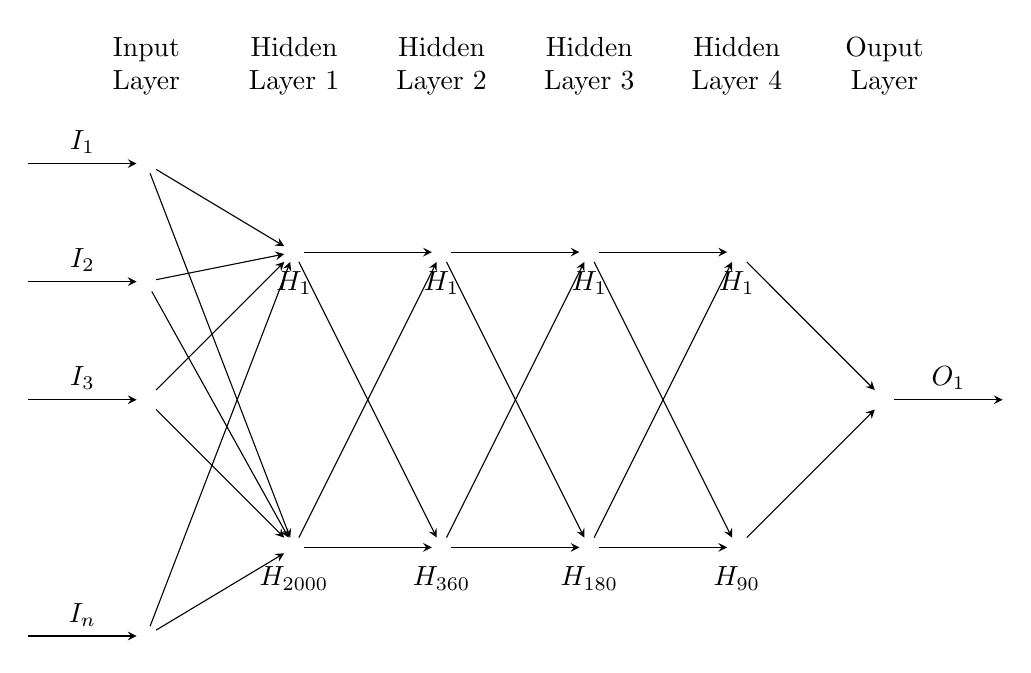
\begin{tikzpicture}[x=1.5cm, y=1.5cm, >=stealth]

\foreach \m/\l [count=\y] in {1,2,3,missing,4}
  \node [every neuron/.try, neuron \m/.try] (input-\m) at (0,2.5-\y) {};

\foreach \m [count=\y] in {1,missing,2}
  \node [every neuron/.try, neuron \m/.try ] (1-hidden-\m) at (1.25,2-\y*1.25) {};

\foreach \m [count=\y] in {1,missing,2}
  \node [every neuron/.try, neuron \m/.try ] (2-hidden-\m) at (2.5,2-\y*1.25) {};
  
 \foreach \m [count=\y] in {1,missing,2}
  \node [every neuron/.try, neuron \m/.try ] (3-hidden-\m) at (3.75,2-\y*1.25) {};

\foreach \m [count=\y] in {1,missing,2}
  \node [every neuron/.try, neuron \m/.try ] (4-hidden-\m) at (5,2-\y*1.25) {};
  
  
\foreach \m [count=\y] in {1}
  \node [every neuron/.try, neuron \m/.try ] (output-\m) at (6.25,\y-1.5) {};

\foreach \l [count=\i] in {1,2,3,n}
  \draw [<-] (input-\i) -- ++(-1,0)
    node [above, midway] {$I_\l$};

\foreach \l [count=\i] in {1,2000}
  \node [below] at (1-hidden-\i.south) {$H_{\l}$};
  
  \foreach \l [count=\i] in {1,360}
  \node [below] at (2-hidden-\i.south) {$H_{\l}$};

\foreach \l [count=\i] in {1,180}
  \node [below] at (3-hidden-\i.south) {$H_{\l}$};

\foreach \l [count=\i] in {1,90}
  \node [below] at (4-hidden-\i.south) {$H_{\l}$};
  
  
\foreach \l [count=\i] in {1}
  \draw [->] (output-\i) -- ++(1,0)
    node [above, midway] {$O_\l$};

\foreach \i in {1,...,4}
  \foreach \j in {1,...,2}
    \draw [->] (input-\i) -- (1-hidden-\j);

\foreach \i in {1,...,2}
  \foreach \j in {1,...,2}
    \draw [->] (1-hidden-\i) -- (2-hidden-\j);

\foreach \i in {1,...,2}
  \foreach \j in {1,...,2}
    \draw [->] (2-hidden-\i) -- (3-hidden-\j);

\foreach \i in {1,...,2}
  \foreach \j in {1,...,2}
    \draw [->] (3-hidden-\i) -- (4-hidden-\j);

    
\foreach \i in {1,...,2}
  \foreach \j in {1}
    \draw [->] (4-hidden-\i) -- (output-\j);

\foreach \l [count=\x from 0] in {Input\\Layer, Hidden\\Layer 1, Hidden\\Layer 2, Hidden\\Layer 3, Hidden\\Layer 4, Ouput\\Layer}
  \node [align=center, above] at (\x*1.25,2) {\l};

\end{tikzpicture}
\caption{Fully connected χωρίς τα επίπεδα Dropout.}
\label{fig:FC_Arch}
\end{figure}

\subsubsection{Επίπεδο Dropout}
Με απλά λόγια, η λειτουργία του επιπέδου Dropout, είναι η απενεργοποίηση, με τυχαίο τρόπο, νευρώνων του προγηούμενου επιπέδου. Το επίπεδο αυτό, έχει μία υπερπαράμετρο, το \textit{Dropout Rate} (DR), το οποίο καθορίζει το πλήθος των νευρώνων που απενεργοποιούνται σε κάθε εποχή (ένα πέρασμα ολόκληρου του dataset από το νευρωνικό). Για παράδειγμα, για $DR=0.4$, με το προηγούμενο επίπεδο να έχει 2000 νευρώνες, σε κάθε εποχή απενεργοποιούνται οι $2000*0.4 = 800$ από αυτούς. Το αποτέλεσμα αυτής της διαδικασίας, είναι το νευρωνικό να μην βασίζεται αποκλειστικά σε μερικούς νευρώνες εκ του συνόλου για την τελική εκτίμηση που δίνει στην έξοδο μειώνοντας με αυτόν τον τρόπο σημαντικά το overfitting. Μια συνοπτική περιγραφή της λειτουργίας του επιπέδου, φαίνεται στο Σχήμα \ref{fig:dropout_ex}. Σε αυτό το σχήμα θεωρείται πως υπάρχει ένα Dropout Layer ενδιάμεσα από όλα τα επίπεδα.

\begin{figure}
\centering
\scalebox{.8}{
\hbox{\hspace{-2em}
\begin{tikzpicture}

	\node[circle, draw, thick] (i1) {};
	\node[circle, draw, thick, above=2em of i1] (i2) {};
	\node[circle, draw, thick, above=2em of i2] (i3) {};
	\node[circle, draw, thick, below=2em of i1] (i4) {};
	\node[circle, draw, thick, below=2em of i4] (i5) {};
	
	\node[circle, draw, thick, right=4em of i1] (h1) {};
	\node[circle, draw, thick, right=4em of i2] (h2) {};
	\node[circle, draw, thick, right=4em of i3] (h3) {};
	\node[circle, draw, thick, right=4em of i4] (h4) {};
	\node[circle, draw, thick, right=4em of i5] (h5) {};
	
	\node[circle, draw, thick, right=4em of h1] (hh1) {};
	\node[circle, draw, thick, right=4em of h2] (hh2) {};
	\node[circle, draw, thick, right=4em of h3] (hh3) {};
	\node[circle, draw, thick, right=4em of h4] (hh4) {};
	\node[circle, draw, thick, right=4em of h5] (hh5) {};
	
	\node[circle, draw, thick, right=4em of hh2] (o1) {};
	\node[circle, draw, thick, right=4em of hh4] (o2) {};
	
	\draw[-stealth, thick] (i1) -- (h1);
	\draw[-stealth, thick] (i1) -- (h2);
	\draw[-stealth, thick] (i1) -- (h3);
	\draw[-stealth, thick] (i1) -- (h4);
	\draw[-stealth, thick] (i1) -- (h5);
	\draw[-stealth, thick] (i2) -- (h1);
	\draw[-stealth, thick] (i2) -- (h2);
	\draw[-stealth, thick] (i2) -- (h3);
	\draw[-stealth, thick] (i2) -- (h4);
	\draw[-stealth, thick] (i2) -- (h5);
	\draw[-stealth, thick] (i3) -- (h1);
	\draw[-stealth, thick] (i3) -- (h2);
	\draw[-stealth, thick] (i3) -- (h3);
	\draw[-stealth, thick] (i3) -- (h4);
	\draw[-stealth, thick] (i3) -- (h5);
	\draw[-stealth, thick] (i4) -- (h1);
	\draw[-stealth, thick] (i4) -- (h2);
	\draw[-stealth, thick] (i4) -- (h3);
	\draw[-stealth, thick] (i4) -- (h4);
	\draw[-stealth, thick] (i4) -- (h5);
	\draw[-stealth, thick] (i5) -- (h1);
	\draw[-stealth, thick] (i5) -- (h2);
	\draw[-stealth, thick] (i5) -- (h3);
	\draw[-stealth, thick] (i5) -- (h4);
	\draw[-stealth, thick] (i5) -- (h5);
	
	\draw[-stealth, thick] (h1) -- (hh1);
	\draw[-stealth, thick] (h1) -- (hh2);
	\draw[-stealth, thick] (h1) -- (hh3);
	\draw[-stealth, thick] (h1) -- (hh4);
	\draw[-stealth, thick] (h1) -- (hh5);
	\draw[-stealth, thick] (h2) -- (hh1);
	\draw[-stealth, thick] (h2) -- (hh2);
	\draw[-stealth, thick] (h2) -- (hh3);
	\draw[-stealth, thick] (h2) -- (hh4);
	\draw[-stealth, thick] (h2) -- (hh5);
	\draw[-stealth, thick] (h3) -- (hh1);
	\draw[-stealth, thick] (h3) -- (hh2);
	\draw[-stealth, thick] (h3) -- (hh3);
	\draw[-stealth, thick] (h3) -- (hh4);
	\draw[-stealth, thick] (h3) -- (hh5);
	\draw[-stealth, thick] (h4) -- (hh1);
	\draw[-stealth, thick] (h4) -- (hh2);
	\draw[-stealth, thick] (h4) -- (hh3);
	\draw[-stealth, thick] (h4) -- (hh4);
	\draw[-stealth, thick] (h4) -- (hh5);
	\draw[-stealth, thick] (h5) -- (hh1);
	\draw[-stealth, thick] (h5) -- (hh2);
	\draw[-stealth, thick] (h5) -- (hh3);
	\draw[-stealth, thick] (h5) -- (hh4);
	\draw[-stealth, thick] (h5) -- (hh5);
	
	
	\draw[-stealth, thick] (hh1) -- (o1);
	\draw[-stealth, thick] (hh1) -- (o2);
	\draw[-stealth, thick] (hh2) -- (o1);
	\draw[-stealth, thick] (hh2) -- (o2);
	\draw[-stealth, thick] (hh3) -- (o1);
	\draw[-stealth, thick] (hh3) -- (o2);
	\draw[-stealth, thick] (hh4) -- (o1);
	\draw[-stealth, thick] (hh4) -- (o2);
	\draw[-stealth, thick] (hh5) -- (o1);
	\draw[-stealth, thick] (hh5) -- (o2);
	
	\draw[-stealth, double, dashed, thick] (5.5,0) -- node[above] {dropout} (8.6, 0);
	
	
	%%% BOUNDARY %%%
	
	\node[circle, draw, thick, red, fill=red!10, right=15em of hh1] (i1) {};
	\node[circle, draw, thick, red, fill=red!10, above=2em of i1] (i2) {};
	\node[circle, draw, thick, above=2em of i2] (i3) {};
	\node[circle, draw, thick, below=2em of i1] (i4) {};
	\node[circle, draw, thick, below=2em of i4] (i5) {};
	
	\node[red] (icr) at (i1) {$\mathlarger{\mathlarger{\mathlarger{\mathlarger{\mathlarger{\bm{\times}}}}}}$};
	\node[red] (icr) at (i2) {$\mathlarger{\mathlarger{\mathlarger{\mathlarger{\mathlarger{\bm{\times}}}}}}$};
	
	\node[circle, draw, thick, red, fill=red!10, right=4em of i1] (h1) {};
	\node[circle, draw, thick, right=4em of i2] (h2) {};
	\node[circle, draw, thick, red, fill=red!10, right=4em of i3] (h3) {};
	\node[circle, draw, thick, red, fill=red!10, right=4em of i4] (h4) {};
	\node[circle, draw, thick, right=4em of i5] (h5) {};
	
	\node[red] (icr) at (h1) {$\mathlarger{\mathlarger{\mathlarger{\mathlarger{\mathlarger{\bm{\times}}}}}}$};
	\node[red] (icr) at (h3) {$\mathlarger{\mathlarger{\mathlarger{\mathlarger{\mathlarger{\bm{\times}}}}}}$};
	\node[red] (icr) at (h4) {$\mathlarger{\mathlarger{\mathlarger{\mathlarger{\mathlarger{\bm{\times}}}}}}$};
	
	\node[circle, draw, thick, right=4em of h1] (hh1) {};
	\node[circle, draw, thick, red, fill=red!10, right=4em of h2] (hh2) {};
	\node[circle, draw, thick, right=4em of h3] (hh3) {};
	\node[circle, draw, thick, red, fill=red!10, right=4em of h4] (hh4) {};
	\node[circle, draw, thick, right=4em of h5] (hh5) {};
	
	\node[red] (icr) at (hh2) {$\mathlarger{\mathlarger{\mathlarger{\mathlarger{\mathlarger{\bm{\times}}}}}}$};
	\node[red] (icr) at (hh4) {$\mathlarger{\mathlarger{\mathlarger{\mathlarger{\mathlarger{\bm{\times}}}}}}$};
	
	\node[circle, draw, thick, right=4em of hh2] (o1) {};
	\node[circle, draw, thick, right=4em of hh4] (o2) {};
	
	\draw[-stealth, thick] (i3) -- (h2);
	\draw[-stealth, thick] (i3) -- (h5);
	\draw[-stealth, thick] (i4) -- (h2);
	\draw[-stealth, thick] (i4) -- (h5);
	\draw[-stealth, thick] (i5) -- (h2);
	\draw[-stealth, thick] (i5) -- (h5);
	
	\draw[-stealth, thick] (h2) -- (hh1);
	\draw[-stealth, thick] (h2) -- (hh3);
	\draw[-stealth, thick] (h2) -- (hh5);
	\draw[-stealth, thick] (h5) -- (hh1);
	\draw[-stealth, thick] (h5) -- (hh3);
	\draw[-stealth, thick] (h5) -- (hh5);
	
	\draw[-stealth, thick] (hh1) -- (o1);
	\draw[-stealth, thick] (hh1) -- (o2);
	\draw[-stealth, thick] (hh3) -- (o1);
	\draw[-stealth, thick] (hh3) -- (o2);
	\draw[-stealth, thick] (hh5) -- (o1);
	\draw[-stealth, thick] (hh5) -- (o2);

\end{tikzpicture}}}
\caption{Περιγραφή της λειτουργίας του Dropout Layer.}
\label{fig:dropout_ex}
\end{figure}

\subsection{Convolutional}
Η CNN αρχιτεκτονική που χρησιμοποιήθηκε σε αυτή την εργασία, αποτελείται από 6 1D-Convolutional επίπεδα, κάθε ένα από τα οποία ακολουθείται από ένα επίπεδο υποδειγματοληψίας, κοινώς γνωστό ως MaxPooling Layer. Πριν το επίπεδο εξόδου υπάρχει ένα πλήρως διασυνδεδεμένο επίπεδο. Όπως και στο προηγούμενο μοντέλο, έτσι και εδώ, όλα τα επίπεδα που περιέχουν νευρώνες, χρησιμοποιούν την ReLU (Εξίσωση \ref{eq:ReLU}) ως συνάρτηση ενεργοποίησης. Χρησιμοποιείται επίσης η τεχνική της μείωσης του ρυθμού μάθησης, όταν ο αλγόριθμος φτάνει σε κάποιο \textit{plateau}, δηλαδή το σφάλμα μένει σταθερό για ένα ορισμένο διάστημα. Και σε αυτή την περίπτωση, η εκπαίδευση έγινε χρησιμοποιώντας, όπως έχει ήδη αναφερθεί, ως συνάρτηση απώλειας το MSE, και τον βελτιστοποιητή Adam (Adaptive Moment Estimation) με αρχικό ρυθμό μάθησης $Lr = 0.001$. Το μοντέλο απεικονίζεται στο Σχήμα \ref{fig:CNN_Arch}. Τα συνελικτικά επίπεδα, αποτελούνται ανά δύο από 128, 64 και 32 φίλτρα μήκους 3, ενώ το πλήρως διασυνδεδεμένο επίπεδο αποτελείται από 180 νευρώνες. 

Η διαδικασία Max Pooling, που αναφέρεται σε αυτή την ενότητα, είναι μια διαδικασία διακριτοποίησης, βασισμένη στα δείγματα. Ο στόχος της είναι η υποδειγματοληψία της αναπαράστασης που δέχεται στην είσοδο, μειώνοντας τις διαστάσεις της. Πρακτικά, αν οριστεί μέγεθος pooling $pool\;size = 3$, τότε το διάνυσμα εισόδου, μήκους $L$, προσπελάζεται με βήμα $pool\;size$, και από κάθε διάστημα τριών δειγμάτων διατηρείται μόνο το μέγιστο. Το αποτέλεσμα είναι ένα διάνυσμα μήκους $\frac{L}{pool size}$.  Όταν αυτό ανάγεται στις δύο διαστάσεις, γίνεται ευκολότερα κατανοητό, όπως παρουσιάζεται στο Σχήμα \ref{fig:max_pooling_2d}.

\begin{figure}[h]
  \centering
  \includegraphics[width=\textwidth]{images/max_pooling_2d.png}
  \caption{Αναγωγή του Max Pooling σε δύο διαστάσεις.}
  \label{fig:max_pooling_2d}
\end{figure}

\begin{figure}[h]
  \centering
  \includegraphics[width=\textwidth]{images/CNN_Arch.png}
  \caption{Η αρχιτεκτονική του μοντέλου CNN για εκτίμηση DOA.}
  \label{fig:CNN_Arch}
\end{figure}